\documentclass[border=6pt]{standalone}
% Shared preamble for web figures.  Each figure is a standalone .tex that
% \input's this file; scripts/make-figures.sh turns it into an SVG.
% Handouts pull the same file with \fig{Unit_X/<name>}.
\usepackage[T1]{fontenc}
\usepackage{helvet}
\renewcommand{\familydefault}{\sfdefault}
\renewcommand{\ttdefault}{pcr}  % Courier: a real Type 1 typewriter font
\usepackage{amsmath}
\usepackage{tikz}
\usetikzlibrary{arrows.meta,positioning,calc,shapes.symbols,shapes.geometric}

% Who makes the rules is the point of most diagrams in this book, so the
% colors mean the same thing everywhere: blue is a person, orange is the
% computer, green is an answer, pink is the human brain.
\definecolor{person}{HTML}{2C6FAE}
\definecolor{machine}{HTML}{D35400}
\definecolor{result}{HTML}{1E8449}
\definecolor{brainpink}{HTML}{C2185B}
\definecolor{ink}{HTML}{2C3E50}

\tikzset{
  doodle/.style={line width=1.5pt, line cap=round, line join=round, draw=ink},
  box/.style={draw, rounded corners=5pt, line width=1.1pt, align=center,
              inner sep=7pt, minimum height=1.0cm, font=\small},
  personbox/.style={box, draw=person, fill=person!10},
  machinebox/.style={box, draw=machine, fill=machine!10},
  resultbox/.style={box, draw=result, fill=result!10},
  plainbox/.style={box, draw=ink!70, fill=ink!4},
  flow/.style={-{Stealth[length=8pt]}, line width=1.4pt, draw=ink},
}

% A person (blue) and a robot head (orange) as small icons.
% \personicon{x}{y}{scale}   \roboticon{x}{y}{scale}
\newcommand{\personicon}[3]{%
  \begin{scope}[shift={(#1,#2)}, scale=#3]
    \fill[person] (0,0.62) circle (0.28);
    \fill[person, rounded corners=6pt] (-0.42,-0.55) rectangle (0.42,0.28);
  \end{scope}}
\newcommand{\roboticon}[3]{%
  \begin{scope}[shift={(#1,#2)}, scale=#3]
    \draw[machine, line width=1.2pt] (0,0.5) -- (0,0.72);
    \fill[machine] (0,0.78) circle (0.08);
    \draw[machine, line width=1.4pt, fill=machine!12, rounded corners=4pt] (-0.5,-0.45) rectangle (0.5,0.5);
    \fill[ink] (-0.2,0.12) circle (0.08);
    \fill[ink] (0.2,0.12) circle (0.08);
    \draw[ink, line width=1pt] (-0.22,-0.22) -- (0.22,-0.22);
  \end{scope}}

\usetikzlibrary{backgrounds}
\begin{document}
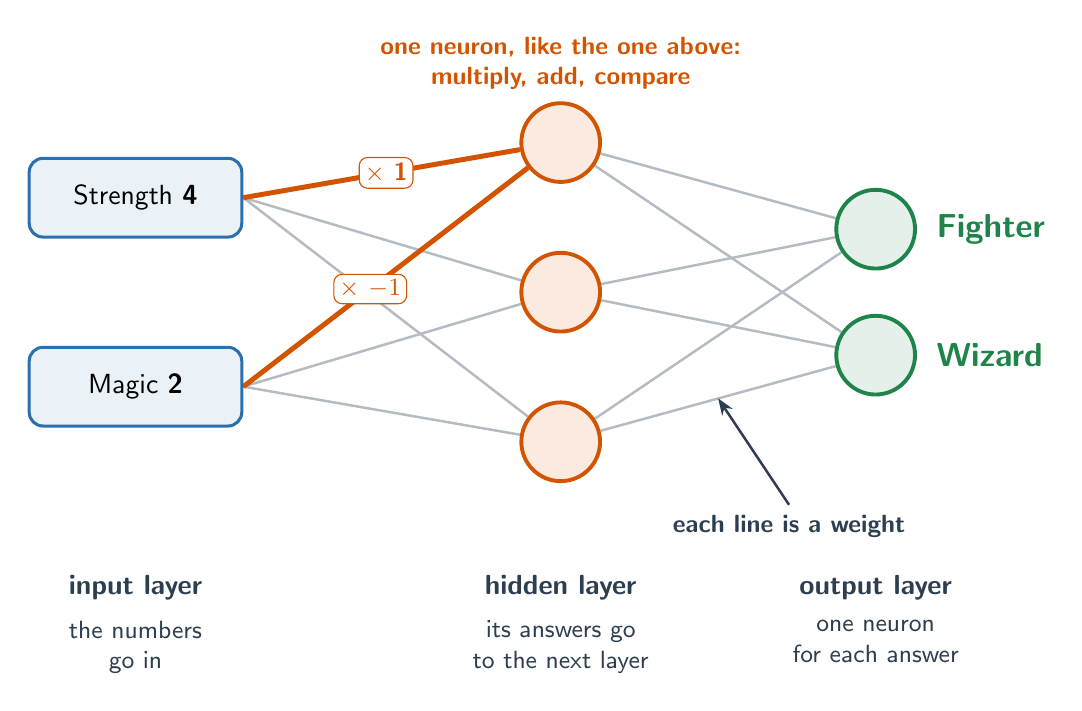
\begin{tikzpicture}[
  inp/.style={personbox, minimum width=2.7cm, font=\normalsize},
  hid/.style={circle, draw=machine, fill=machine!12, line width=1.4pt, minimum size=1.0cm},
  outn/.style={circle, draw=result, fill=result!12, line width=1.4pt, minimum size=1.0cm},
  wire/.style={draw=ink!35, line width=0.9pt},
  hot/.style={draw=machine, line width=1.8pt},
  wt/.style={fill=white, draw=machine, rounded corners=3pt, font=\small\bfseries, text=machine, inner sep=2pt},
  laycap/.style={font=\normalsize\bfseries, text=ink, align=center},
  laysub/.style={font=\small, text=ink, align=center, anchor=north},
]
% A small neural network: 2 inputs, a hidden layer of 3 neurons, 2 outputs.
% The top hidden neuron is the neuron from 2.4.1 (same inputs, same weights).
\node[inp] (i1) at (0,2.9) {Strength \textbf{4}};
\node[inp] (i2) at (0,0.5) {Magic \textbf{2}};
\foreach \j/\y in {1/3.6, 2/1.7, 3/-0.2} \node[hid] (h\j) at (5.4,\y) {};
\node[outn] (o1) at (9.4,2.5) {};
\node[outn] (o2) at (9.4,0.9) {};
\node[font=\large\bfseries, text=result, anchor=west] at (10.05,2.5) {Fighter};
\node[font=\large\bfseries, text=result, anchor=west] at (10.05,0.9) {Wizard};

% every line is a weight
\begin{scope}[on background layer]
  \foreach \i in {1,2} \foreach \j in {2,3} \draw[wire] (i\i.east) -- (h\j);
  \foreach \j in {1,2,3} \foreach \k in {1,2} \draw[wire] (h\j) -- (o\k);
  \draw[hot] (i1.east) -- (h1); \draw[hot] (i2.east) -- (h1);
\end{scope}
\node[wt] at ($(i1.east)!0.45!(h1)$) {$\times$ 1};
\node[wt] at ($(i2.east)!0.4!(h1)$) {$\times$ $-1$};
\node[font=\small\bfseries, text=machine, align=center, anchor=south] at (5.4,4.15) {one neuron, like the one above:\\multiply, add, compare};

% point at one plain line
\coordinate (w) at ($(h3)!0.5!(o2)$);
\draw[ink, line width=0.9pt, -{Stealth[length=6pt]}] (8.3,-1.0) node[anchor=north, font=\small\bfseries, text=ink] {each line is a weight} -- (w);

% the layers
\foreach \x/\c/\s in {0/input layer/the numbers\\go in, 5.4/hidden layer/its answers go\\to the next layer, 9.4/output layer/one neuron\\for each answer} {
  \node[laycap] at (\x,-2.05) {\c};
  \node[laysub] at (\x,-2.35) {\s};
}
\end{tikzpicture}
\end{document}
